
\section{The ICA problem}

\begin{frame}{\secname}

Let $\vec s = (s_1, s_2,...,s_N)^\top$ denote the concatenation of $N$ \underline{independent sources} 
and $\vec x \in \R^N$ describe our observations. $\vec x$ relates to $\vec s$ through a 
\emph{linear transformation} $\vec A$:

\begin{equation}
\label{eq:ica}
\vec x = \vec A \, \vec s
\end{equation}

\notesonly{Again with individual elements and }with $N=2$:
\begin{equation}
 \left( \begin{array}{ll}
			x_1 \\ x_2
		\end{array} \right)
        = \left( \begin{array}{ll}
			a_{11} & a_{12} \\ a_{21} & a_{22}
		\end{array} \right) \cdot \left( \begin{array}{ll}
			s_1 \\ s_2
		\end{array} \right)
	= \left( \begin{array}{l}
		a_{11} s_1 + a_{12} s_2 \\ a_{21} s_1 + a_{22} s_2
	\end{array} \right)
\end{equation}

We refer to $\vec A$ as the \emph{mixing matrix} and \notesonly{\eqref{eq:ica}}\slidesonly{the above} as the \emph{ICA problem}, 
which is recovering $\vec s$ from only observing $\vec x$.

\end{frame}

\begin{frame}{\secname}

The ICA problem can be solved by finding the \emph{unmixing matrix} $\vec W$ such that 
\begin{equation}
\vec s = \vec W \cdot \vec x = \vec A^{-1} \cdot \vec x
\end{equation}

But since we don't have the original mixing matrix $\vec A$ we employ methods of ICA for finding an unmixing matrix $\vec W$ which yields an estimate of the sources, namely $\vec {\hat s}$. 

\begin{equation}
\hat{\vec s} = \vec W \cdot \vec x = \vec A^{-1} \cdot \vec x
\end{equation}

In the case of $N=2$:

\begin{equation}
 \left( \begin{array}{ll}
			\hat s_1 \\ \hat s_2
		\end{array} \right)
        = \left( \begin{array}{ll}
			w_{11} & w_{12} \\ w_{21} & w_{22}
		\end{array} \right) \cdot \left( \begin{array}{ll}
			x_1 \\ x_2
		\end{array} \right)
	= \left( \begin{array}{l}
		w_{11} x_1 + w_{12} x_2 \\ w_{21} x_1 + w_{22} x_2
	\end{array} \right)
\end{equation}

\end{frame}

\begin{frame}{Different methods for solving the ICA problem}

\notesonly{We will discuss several methods for solving the ICA problem:}

\begin{itemize}
\item Methods that maximize the \emph{mutual information} between the observations $\vec x$ and the estimated sources $\vec {\hat s}$ (e.g. Infomax)
\item Methods for maximizing the \emph{non-gaussianity} of $\vec {\hat s}$ (e.g. Kurtosis-based ICA, FastICA)
\end{itemize}

\end{frame}

\begin{frame}{Infomax - Overview}


\clearpage

\underline{Outline for \emph{Infomax} ICA}:
\begin{itemize}
	\item \notesonly{We first look into some }key concepts:
    \begin{itemize}
		\item Uncorrelatedness
		\item \emph{statistical independence}
    \end{itemize}
    \item A primer on information theory
    \begin{itemize}
        \item Entropy
        \item Conditional Entropy
        \item Relative Entropy or \emph{Kullback-Leibler (KL) divergence}
        \item Mutual Information
    \end{itemize}
    \item cost function
    \item ERM
    \item practical aspects
\end{itemize}

\end{frame}

\subsection{Uncorrelatedness}

\begin{frame}{\subsecname}

Correlation measures the linear relationship between two random variables.
\begin{center}
\includegraphics[width=0.7\textwidth]{img/section2_fig3.pdf}
\notesonly{\captionof{figure}{Correlation and uncorrelatedness}}
\end{center}

If no such correlation exists between two random scalar variables $X_1$ and $X_2$. That is, if

\svspace{-3mm}

\begin{align}
\label{eq:uncorr}
\mathrm{Cov}(X_1, X_2) = \E  \lbrack X_1  X_2 \rbrack - \E  \lbrack X_1 \rbrack \, \E \lbrack X_2 \rbrack  &= 0\\
\E  \lbrack X_1  X_2 \rbrack &= \E  \lbrack X_1 \rbrack \, \E \lbrack X_2 \rbrack
\end{align}

$\Rightarrow$ The two variables are \emph{uncorrelated}.

\end{frame}

\subsection{Statistical independence}

\begin{frame}{\subsecname}

Consider the following two random scalar variables $X$ and $Y$:
\begin{center}
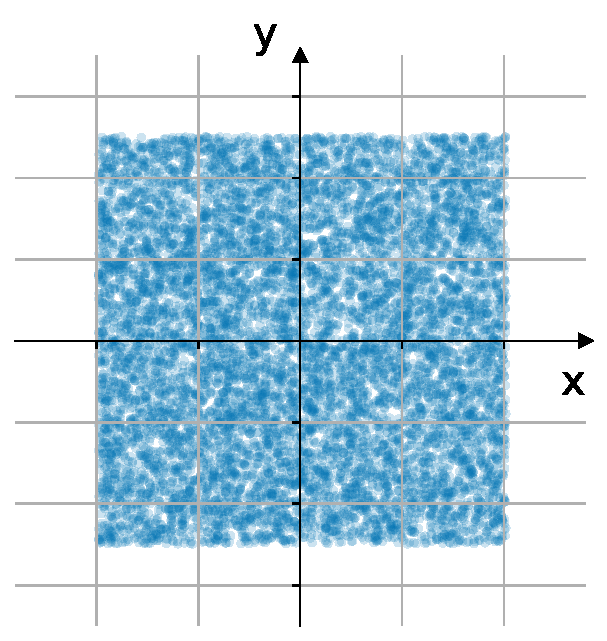
\includegraphics[width=0.4\textwidth]{img/uniform_fixed}
\end{center}

Knowing anything about $X$ reveals absolutely nothing about $Y$, and vice-versa. This is because both variables are \emph{independent}. 

\end{frame}

\begin{frame}{\subsecname}

\only<1>{
Independence requires that the joint probability $p_{X,Y}(x,y)$ factorizes into the product of 
the marginal probabilities $p_X(x)$ and  $p_Y(y)$:

\begin{equation}
\label{eq:statindep}
p_{X,Y}(x,y) = p_X(x) p_Y(y)
\end{equation}

From this follows:
}
\only<1,2>{

\begin{equation}
\label{eq:statindepexp}
\E  \lbrack \, g(x) h(y) \, \rbrack = \E \lbrack g(x) \rbrack \, \E \lbrack h(y) \rbrack  \,,
\end{equation}

where $g(x)$ and $h(y)$ are absolutely integrable functions of $X$ and $Y$.
}
\only<2>{


This can be shown with\notesonly{ the use of \eqref{eq:statindep}}:

\begin{align}
\E  \lbrack \, g(x) h(y) \, \rbrack &= \int_{-\infty}^{\infty} \int_{-\infty}^{\infty} g(x) \, h(y) \, p_{X,Y}(x,y) \, dx \, dy \\
&= \int_{-\infty}^{\infty} \int_{-\infty}^{\infty} g(x) \, h(y)  \, p_X(x) \, p_Y(y) \, dx \, dy \\
&= \int_{-\infty}^{\infty}  g(x) \, p_X(x) dx\, \int_{-\infty}^{\infty} h(y) \, p_Y(y) dy
\,.
\end{align}
}

\end{frame}

\begin{frame}{Uncorrelatedness vs. statistical independence}

\notesonly{
Independence is a much stronger property than decorrelatedness. 
}

\slidesonly{
\begin{center}
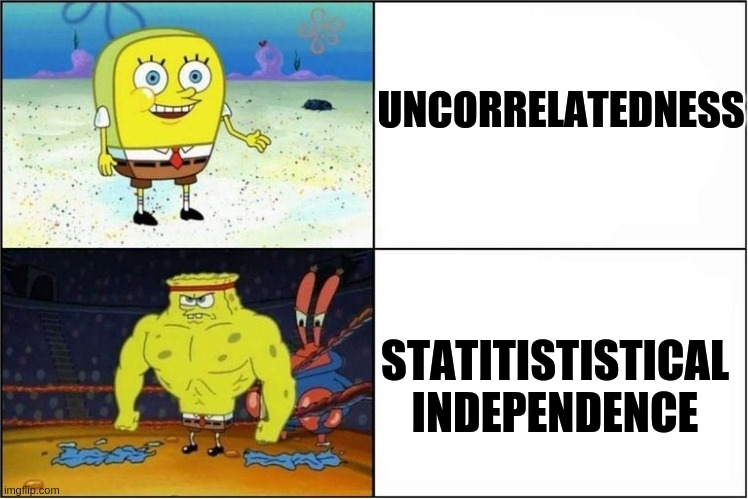
\includegraphics[width=0.4\textwidth]{img/meme_stronger}
\end{center}
}

\pause

If $X$ and $Y$ are independent, they are also uncorrelated, but the same cannot always be said the other way around.



\end{frame}

\begin{frame}{Uncorrelatedness vs. statistical independence}

\only<1>{
Example\footnote{\notesonly{Example obtained} from (Hyv\"arinen, A., \& Oja, E. (2000). Independent component analysis: algorithms and applications. Neural networks, 13(4-5), 411-430.)}:

Assume $X$ and $Y$ are discrete valued and follow a distribution that the pair are with probability 1/4 equal to any of the following
values: (0,1),(0,-1),(1,0),(-1,0). 
}
\begin{center}
	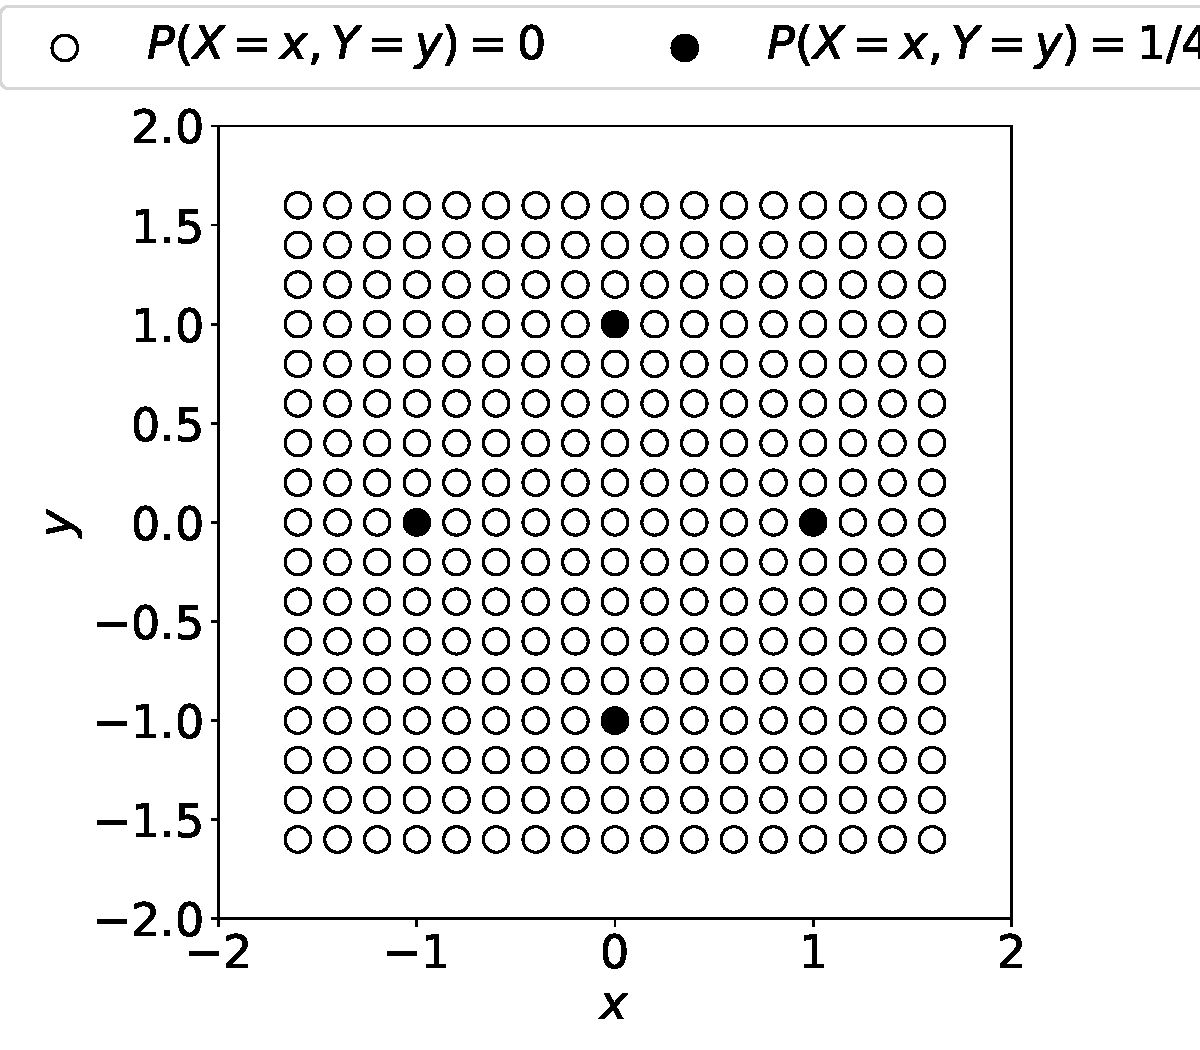
\includegraphics[width=0.4\textwidth]{img/example_decorr_notindep}
	\notesonly{\captionof{figure}{Example for decorrelatedness vs. Independence}}
\end{center}

\only<2-4>{
\question{Are $X$ and $Y$ uncorrelated?}

}
\only<3-4>{

-We check:\\

$\E \lbrack X \rbrack = \frac{1}{4} \cdot (0 + 0 + 1 + (-1)) = 0$\\[2mm]
$\E \lbrack Y \rbrack = \frac{1}{4} \cdot (1 + (-1) + 0 + 0) = 0$\\
}

\notesonly{
- Yes they are uncorrelated.
}

\only<4>{
\slidesonly{
\placeimage{11}{5}{img/meme_yesuncorrelated}{width=3.5cm}
}
}

\end{frame}

\begin{frame}{Uncorrelatedness vs. statistical independence}

\slidesonly{
\begin{center}
	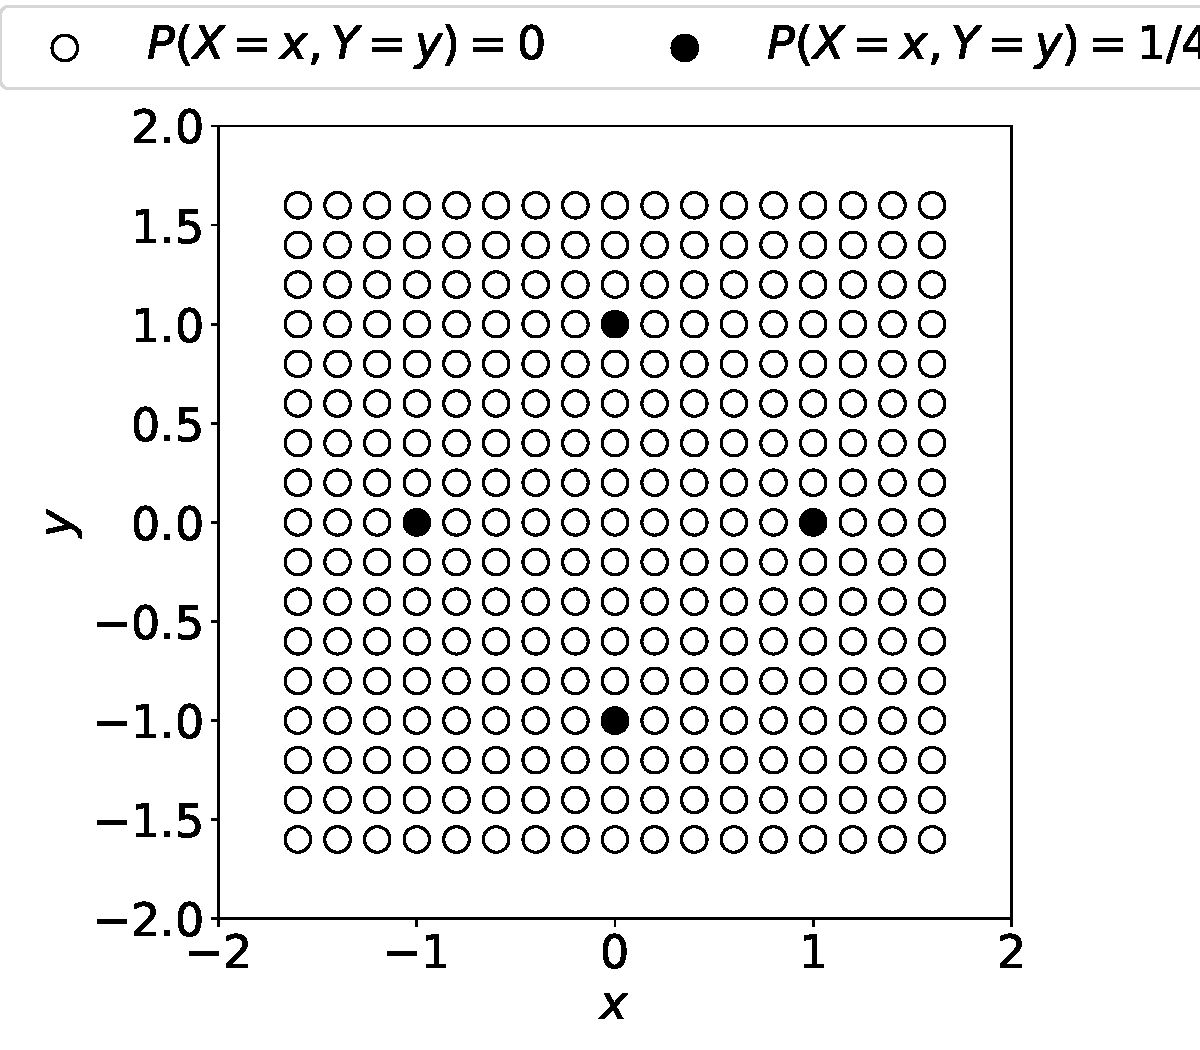
\includegraphics[width=0.4\textwidth]{img/example_decorr_notindep}
	\notesonly{\captionof{figure}{Example for decorrelatedness vs. Independence}}
\end{center}
}

\only<1-3>{
\question{Are $X$ and $Y$ statistically independent?}

}
\only<2-3>{

\notesonly{-As }we calculate $\E  \lbrack \, g(x) h(y) \, \rbrack$ with, e.g., $g(x)=x^2$ and $h(y)=y^2$:\\
$\E \lbrack x^2 \, y^2 \rbrack 
= \frac{1}{4} \cdot \lbrack (0\cdot1) + (0\cdot1) + (1\cdot0) + (1\cdot0) \rbrack = 0 
\ne \frac{1}{4} = \E \lbrack x^2 \rbrack \, \E \lbrack y^2 \rbrack \;,$

\notesonly{we see that }the requirement for independence \notesonly{as in \eqref{eq:statindepexp} }is violated. \notesonly{The variables are uncorrelated but \underline{not} independent.}
}




\only<3>{
\slidesonly{
\placeimage{10.5}{5}{img/meme_butnotindep}{width=4.cm}
}
}

\end{frame}

\clearpage

\begin{frame}

\question{How does statistical independence fit into ICA?}

\pause

- The solution to the ICA problem yields a distribution of the estimated source $\widehat{P}_{\vec s}(\widehat{\vec s})$ that is closest to the factorizing density:

\begin{equation}
\widehat{P}_{s_1, s_2,\ldots,s_N}({\widehat s_1, \widehat s_2,\ldots,\widehat s_N}) = \widehat{P}_{s_1}(\widehat{s_1}) \cdot \widehat{P}_{s_2}(\widehat{s_2}) \cdot \, \ldots \, \cdot \widehat{P}_{s_N}(\widehat{s}_N)
\end{equation}

\pause

\begin{equation}
\label{eq:facts}
\widehat{P}_{\vec s}(\widehat{\vec s}) = \prod_{i=1}^{N} \widehat{P}_{s_i}(\widehat{s_i})  \,.
\end{equation}

To clarify the notation here:\\
\begin{itemize}
%\vspace{-5mm}
%\renewcommand\labelitemi{--}
\setlength\itemsep{0.1em}
\item $\vec s$ describes the independent sources which we do not have.
\item $\widehat{\vec s}$ are the reconstructed sources which we obtain via some unmixing matrix $\vec W$.
\item $\widehat{P}_{\vec s}(\widehat{\vec s})$ is our estimate of the pdf of $\vec s$ which we have approximated using the reconstructions $\widehat{\vec s}$. 
\end{itemize}

\end{frame}
